\documentclass[12pt]{article}
\usepackage[utf8]{inputenc}
\usepackage[T2A]{fontenc}
\usepackage[russian]{babel}
\usepackage[pdftex]{graphicx}
\usepackage{amsmath,amsfonts,amssymb,amsthm,mathtools}
\usepackage{geometry} % Меняем поля страницы
\geometry{left=1.5cm}% левое поле
\geometry{right=2cm}% правое поле
\geometry{top=1cm}% верхнее поле
\geometry{bottom=2cm}% нижнее поле
\graphicspath{{.}}
\DeclareGraphicsExtensions{.pdf,.png,.jpg}

\begin{document}

\begin{titlepage}
\Large

\begin{center}
Санкт-Петербургский \\ Политехнический университет Петра Великого\\
Физико-механический институт\\
ВШТМиМФ

\vspace{12em}

\textbf{Индивидуальная работа №4}

\textbf{Метод конечных элементов. Исследование функций форм}

по дисциплине "Вычислительная механика"
\end{center}

\vspace{6em}

\newbox{\lbox}
\savebox{\lbox}{\hbox{Гришина Юлия Николаевна}}
\newlength{\maxl}
\setlength{\maxl}{\wd\lbox}
\hfill\parbox{14cm}{
\hspace*{5cm}\hspace*{-5cm}Студент:\hfill\hbox to\maxl{Гришина Юлия Николаевна\hfill}\\
\hspace*{5cm}\hspace*{-5cm}Преподаватель:\hfill\hbox to\maxl{Витохин Евгений Юрьевич}\\
\\
\hspace*{5cm}\hspace*{-5cm}Группа:\hfill\hbox to\maxl{5030103/00201}\\
}

\vspace{\fill}

\begin{center}
Санкт-Петербург \\2022
\end{center}

\end{titlepage}

\textbf{Постановка задачи}\\
Дан конечный элемент заданной формы и тип интерполяционного полинома:
\begin{figure}[h]

\centering

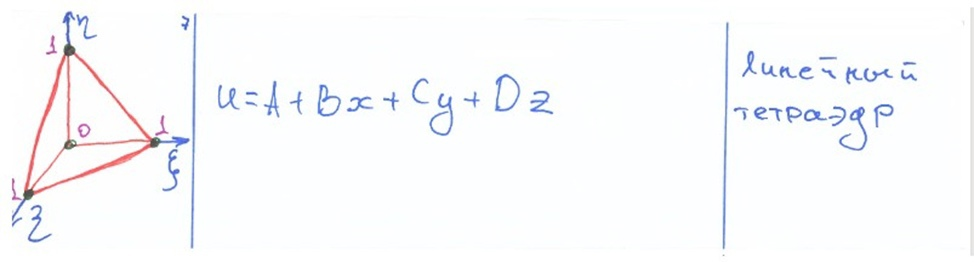
\includegraphics[width=1\linewidth]{0.jpg}

\end{figure}\\
Необходимо найти функции формы для линейного тетраэдра, удовлетворяющие следующим свойствам:\\
$1. \sum N_s (x,y,z) = 1;$\\
$2. N_s (x_m,y_m,z_m) = \begin{cases} 0, s \neq m \\ 1, s=m \end{cases}$\\
и получить графики поверхностей.\\

\textbf{Метод решения}\\
Данная задача решается с помощью метода конечных элементов.\\
Найдем все узловые точки линейного тетраэдра:\\
$1 - (0,0,0); 2 - (1,0,0); 3 - (0,1,0); 4 - (0,0,1).$\\
Можем записать систему:\\
$\begin{cases} N_1(x_1,y_1,z_1) = A_1 + B_1x_1 + C_1y_1 + D_1z_1\\
N_2(x_1,y_1,z_1) = A_2 + B_2x_1 + C_2y_1 + D_2z_1\\
N_3(x_1,y_1,z_1) = A_3 + B_3x_1 + C_3y_1 + D_3z_1\\
N_4(x_1,y_1,z_1) = A_4 + B_4x_1 + C_4y_1 + D_4z_1
\end{cases}$\\
По свойствам функций форм:\\
$\begin{cases} N_1 = 1\\ N_2 = 0\\ N_3 = 0\\ N_4 = 0 \end{cases}$\\
То же самое можем проделать для других узлов:\\
$\begin{cases} N_1(x_2,y_2,z_2) = A_1 + B_1x_2 + C_1y_2 + D_1z_2 = 0\\
N_2(x_2,y_2,z_2) = A_2 + B_2x_2 + C_2y_2 + D_2z_2 = 1\\
N_3(x_2,y_2,z_2) = A_3 + B_3x_2 + C_3y_2 + D_3z_2 = 0\\
N_4(x_2,y_2,z_2) = A_4 + B_4x_2 + C_4y_2 + D_4z_2 = 0
\end{cases}$\\
$\begin{cases} N_1(x_3,y_3,z_3) = A_1 + B_1x_3 + C_1y_3 + D_1z_3 = 0\\
N_2(x_3,y_3,z_3) = A_2 + B_2x_3 + C_2y_3 + D_2z_3 = 0\\
N_3(x_3,y_3,z_3) = A_3 + B_3x_3 + C_3y_3 + D_3z_3 = 1\\
N_4(x_3,y_3,z_3) = A_4 + B_4x_3 + C_4y_3 + D_4z_3 = 0
\end{cases}$\\
$\begin{cases} N_1(x_4,y_4,z_4) = A_1 + B_1x_4 + C_1y_4 + D_1z_4 = 0\\
N_2(x_4,y_4,z_4) = A_2 + B_2x_4 + C_2y_4 + D_2z_4 = 0\\
N_3(x_4,y_4,z_4) = A_3 + B_3x_4 + C_3y_4 + D_3z_4 = 0\\
N_4(x_4,y_4,z_4) = A_4 + B_4x_4 + C_4y_4 + D_4z_4 = 1
\end{cases}$\\
В матричном виде получим:\\
\[X \cdot A = E\]
Иначе:\\
\[\begin{bmatrix}
1& x_1& y_1& z_1\\
1& x_2& y_2& z_2\\
1& x_3& y_3& z_3\\
1& x_4& y_4& z_4
\end{bmatrix} \cdot
\begin{bmatrix}
A_1& A_2& A_3& A_4\\
B_1& B_2& B_3& B_4\\
C_1& C_2& C_3& C_4\\
D_1& D_2& D_3& D_4
\end{bmatrix} = E\]
Где $(x_1, y_1, z_1) = (0,0,0); (x_2, y_2, z_2) = (1,0,0); (x_3, y_3, z_3) = (0,1,0); (x_4, y_4, z_4) = (0,0,1).$\\
По определению:\\
\[A \cdot A^{-1} = E\]
А значит, $A = X^{-1}.$ Таким образом, получим матрицу коэффициентов функций форм.\\
Введем интерполяционный полином:\\
\[\{P\}^T = \{1 \; x \; y \; z\}\]
Тогда функции форм можно найти:\\
\[[N] = \{P\}^T \cdot A\]

\textbf{Результаты}\\
В результате работы программы были получены функции форм для каждого из узлов:\\
$N(x, y, z) = [1 - y - z - x, x, y, z]$\\
$N_1 = 1 - y - z - x$ для узла $(0,0,0)$\\
$N_2 = x$ для узла $(1,0,0)$\\
$N_3 = y$ для узла $(0,1,0)$\\
$N_4 = z$ для узла $(0,0,1)$\\
Проверим выполнение свойств функции формы:\\
$1. N_s (x_m,y_m,z_m) = \begin{cases} 0, s \neq m \\ 1, s=m \end{cases}$\\
$N_1(0,0,0) = 1 - 0 - 0 - 0 = 1$\\
$N_2(1,0,0) = 1$\\
$N_3(0,1,0) = 1$\\
$N_4(0,0,1) = 1$\\
$2. \sum N_s (x,y,z) = 1;$\\
$N_1(x,y,z) + N_2(x,y,z) + N_3(x,y,z) + N_4(x,y,z) = 1.$\\
\newpage
Также построим графики функции форм:\\
\begin{figure}[h]

\centering

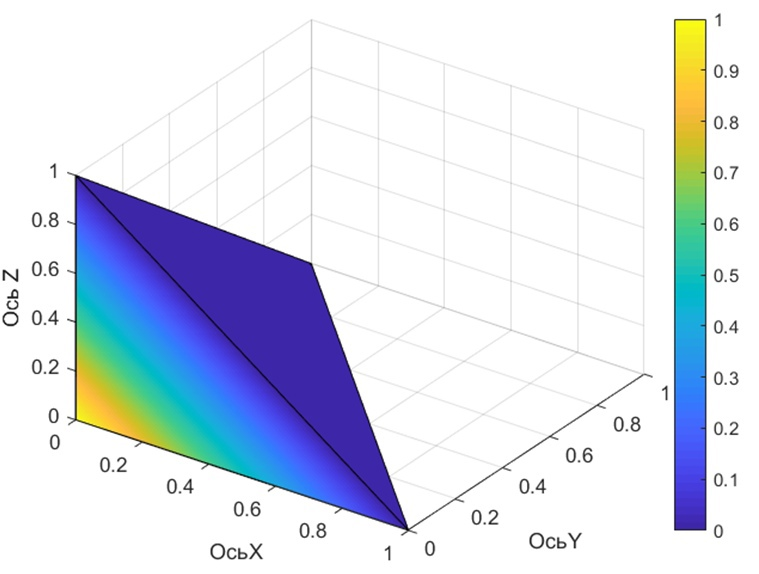
\includegraphics[width=0.6\linewidth]{1.jpg}

\caption{Функция формы $N_1$ в точке $(0,0,0)$}

\label{fig:mpr}

\end{figure}

\begin{figure}[h]

\centering

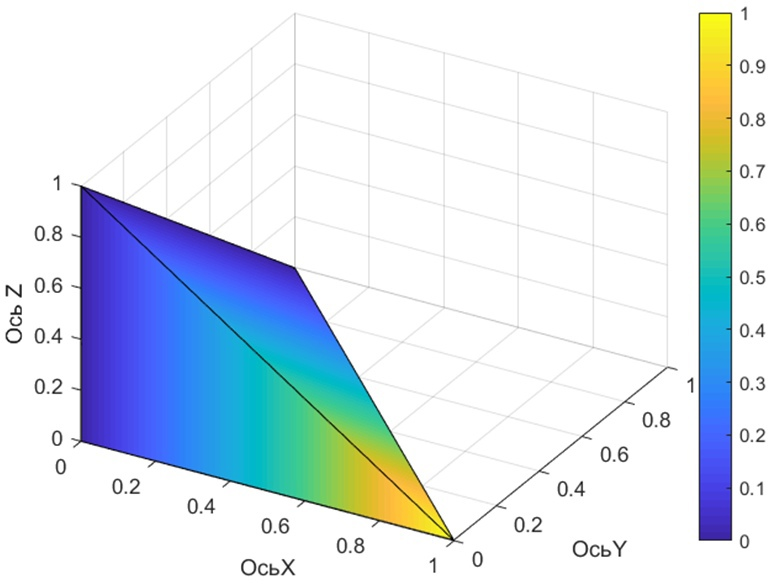
\includegraphics[width=0.6\linewidth]{2.jpg}

\caption{Функция формы $N_2$ в точке $(1,0,0)$}

\label{fig:mpr}

\end{figure}

\newpage
\begin{figure}[h]

\centering

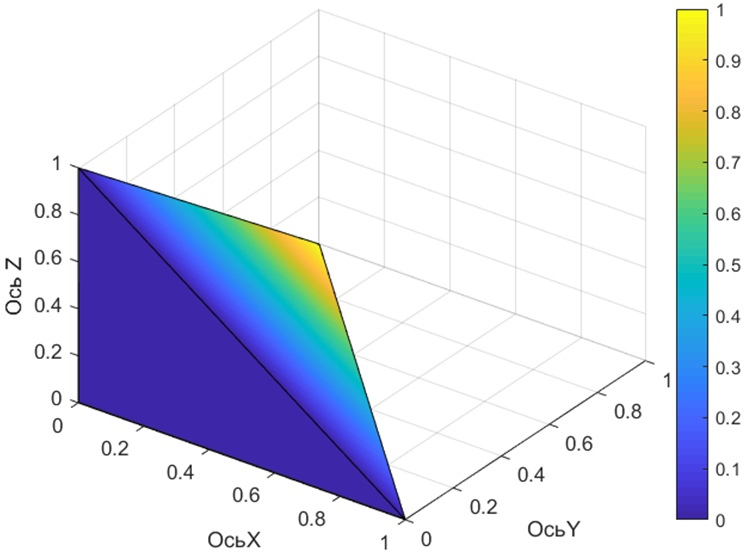
\includegraphics[width=0.6\linewidth]{3.jpg}

\caption{Функция формы $N_3$ в точке $(0,1,0)$}

\label{fig:mpr}

\end{figure}

\begin{figure}[h]

\centering

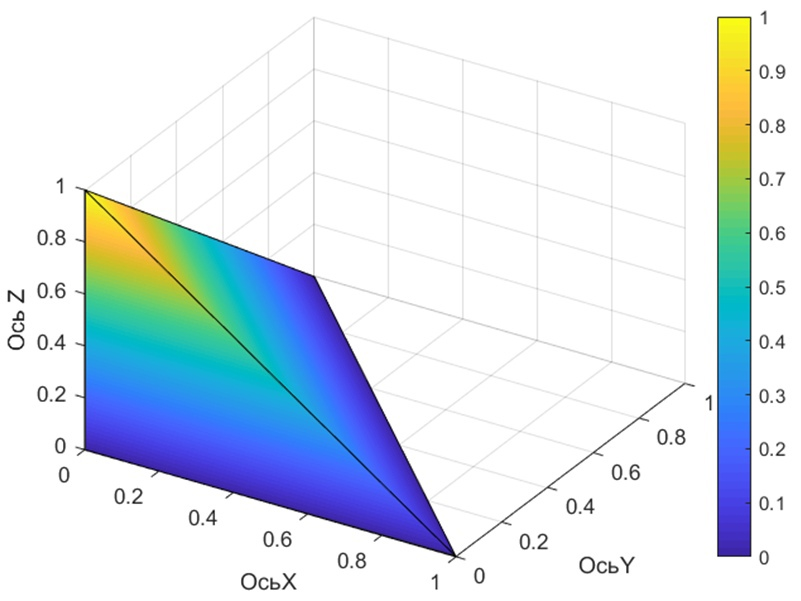
\includegraphics[width=0.6\linewidth]{4.jpg}

\caption{Функция формы $N_4$ в точке $(0,0,1)$}

\label{fig:mpr}

\end{figure}

Таким образом, в ходе работы были найдены функции форм для линейного тетраэдра.\\
Построены графики для соответствующих узлов и проверено выполнение свойства.

\end{document}